\section{Introduction}\label{sec:intro}
A physics system is always described by an action functional (if exist)
\bea
S: \cE \to \bR,
\eea
where $\cE$ is the \emph{space of fields}. The classical physics is described by the critical locus of the action functional:
\bea
\on{Crit}(S)= \lcb \delta S=0\rcb / \sim.
\eea
$\delta S=0$ is called the \emph{equation of motion} which arises from the variation of the action functional $S$. 
$\on{Crit}(S)$
is essentially a set of equivalence classes induced by an arbitrary symmetry. In this lecture, we will focus on the quantum physics. One canonical way to approach the quantum physics is by the {\bf Feynman path integral}:
\bea
\int_\cE e^{iS/\hbar}.
\eea
When $\hbar$ is very small, the above integral
is asymptotically approximated around the critical locus of $S$; this is a method
called the \emph{stationary phase approximation}. The classical limit is obtained by $\hbar\to 0$.

\begin{eg} Here are some basic examples of quantum field theory that we will discuss
throughout this lecture.
\bi[(1)]
\item \textbf{Scalar field theory}. The fields are smooth functions on a manifold $X$.
$\cE=C^\infty(X)$.
\bea
S\lsb \phi\rsb = \int_X |d\phi|^2+m^2\phi^2, \qquad \phi\in C^\infty(X).
\eea

\item \textbf{Gauge theory}. The fields are connections on a vector bundle over $X$, $V\to X$. $\cE=\lcb \text{connections on } V\to X \rcb$.
\bea
\text{Yang-Mills:  } \on{YM}[A] &=\int \Tr F\wedge \ast F, \qquad F=dA+\hf [A,A].\\
\text{Chern-Simons:  } \on{CS}[A] &=\hf\int \Tr A\wedge dA+\frac{1}{6}\int \Tr A\wedge [A,A].
\eea
The Chern-Simons theory is described in 3 dimensions, $\on{dim} X=3$.

\item \textbf{Sigma model}. The fields are maps between two manifolds.
$\cE=\lcb \text{maps } \Sigma \mapsto X \rcb$.

\item \textbf{Gravity}. The fields are metrics on a manifold $X$.
$\cE=\lcb \text{metrics on } X\rcb$.
\ei
\end{eg}

In all the above examples, the space $\cE$ is HUGE in which the integral is an infinite dimensional integral, $\int_\cE (\infty-\text{dim})$. 
In light of this fact, there are (mathematically) no rigorous definitions of the theories in general.
This causes a big trouble in mathematics
to understand quantum physics.
However, in a special region such as the $\hbar$-asymptotic region, a theory exists and is well established, giving rise to the \textbf{perturbative renormalization theory}. 

\subsection*{Observables}
Suppose we consider a quantum field theory (QFT) on a spacetime manifold $X$ and $\cE$ is the space of sections of a vector bundle $E$, $\cE=\Gamma(X,E)$. We want to understand the integral $\int_\cE$.
\bi[(1)]
\item $X=\text{a point}$, $E=$ vector space, say, $\bR^n$, $\cE=\bR^n$. Hence,
$\int_\cE$ leads to the usual calculus that we learnt in high school.

\item $\on{dim} X>0$ (i.e. $X$ is not a point) and there is a fiber $E_p$ (for example, a linear space) at each point $p\in X$. But $\cE\neq \coprod_{p\in X} E_p$; the topology of $X$ makes a difference! This leads to some new structures, known as the \textbf{observable algebras}.
\bea
\tikzset{every picture/.style={line width=0.75pt}} %set default line width to 0.75pt        
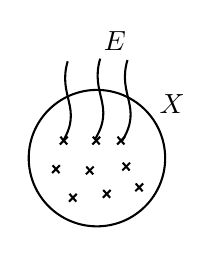
\begin{tikzpicture}[x=0.75pt,y=0.75pt,yscale=-1,xscale=1]
%uncomment if require: \path (0,300); %set diagram left start at 0, and has height of 300

%Flowchart: Connector [id:dp7499007648582767] 
\draw   (102,128.42) .. controls (102,110.26) and (116.72,95.55) .. (134.87,95.55) .. controls (153.02,95.55) and (167.74,110.26) .. (167.74,128.42) .. controls (167.74,146.57) and (153.02,161.29) .. (134.87,161.29) .. controls (116.72,161.29) and (102,146.57) .. (102,128.42) -- cycle ;
%Curve Lines [id:da20650999562395134] 
\draw    (118.28,120.59) .. controls (128.3,104.31) and (115.77,98.68) .. (120.78,81.77) ;
%Curve Lines [id:da9327641008081606] 
\draw    (133.93,119.34) .. controls (143.95,103.06) and (131.43,97.43) .. (136.43,80.52) ;
%Curve Lines [id:da6594075499360046] 
\draw    (147.08,119.97) .. controls (157.1,103.69) and (144.57,98.05) .. (149.58,81.15) ;
%Straight Lines [id:da13073640175251722] 
\draw    (117.25,118.09) -- (120.56,121.84) ;
%Straight Lines [id:da6620526994394944] 
\draw    (117.03,121.84) -- (120.78,118.09) ;

%Straight Lines [id:da8834541176981523] 
\draw    (132.9,118.09) -- (136.21,121.84) ;
%Straight Lines [id:da7510502290287235] 
\draw    (132.68,121.84) -- (136.43,118.09) ;

%Straight Lines [id:da44000068691517] 
\draw    (144.79,118.09) -- (148.11,121.84) ;
%Straight Lines [id:da8590400883175344] 
\draw    (144.57,121.84) -- (148.33,118.09) ;

%Straight Lines [id:da12268308784857629] 
\draw    (113.49,131.86) -- (116.81,135.62) ;
%Straight Lines [id:da22306917883937993] 
\draw    (113.27,135.62) -- (117.03,131.86) ;

%Straight Lines [id:da9728876585033619] 
\draw    (129.77,132.49) -- (133.08,136.24) ;
%Straight Lines [id:da23216656218706566] 
\draw    (129.55,136.24) -- (133.3,132.49) ;

%Straight Lines [id:da8478449055046726] 
\draw    (147.3,130.61) -- (150.61,134.37) ;
%Straight Lines [id:da7584484914378529] 
\draw    (147.08,134.37) -- (150.83,130.61) ;

%Straight Lines [id:da3145627797214947] 
\draw    (121.63,145.63) -- (124.94,149.39) ;
%Straight Lines [id:da696844406939886] 
\draw    (121.41,149.39) -- (125.17,145.63) ;

%Straight Lines [id:da4079053352483115] 
\draw    (137.91,143.76) -- (141.22,147.51) ;
%Straight Lines [id:da867418207840257] 
\draw    (137.69,147.51) -- (141.44,143.76) ;

%Straight Lines [id:da6401735618210065] 
\draw    (153.56,140.63) -- (156.87,144.38) ;
%Straight Lines [id:da7675951895008961] 
\draw    (153.34,144.38) -- (157.1,140.63) ;

% Text Node
\draw (163.62,96.13) node [anchor=north west][inner sep=0.75pt]   [align=left] {$X$};
% Text Node
\draw (136.7,66.07) node [anchor=north west][inner sep=0.75pt]   [align=left] {$E$};
\end{tikzpicture}
\eea
\ei

Roughly speaking, 
observables are functions on fields, denoted as
$\cO(\cE)$ (or certain homology). For example, 
distributions are \emph{linear observables}.

The new structures come from the following fact:
\begin{itemize}
\item Given an open subset $U\subset X$, we can talk about
\bea \on{Obs}(U)= \text{observables supported in U}.\eea

\begin{eg}
$\cE=C^\infty(X),\ p\in X$. Consider 
\bea \cO_1: \cE \to \bR,\eea
where $\cO_1(f)=f(p)^m, \ \forall f\in \cE$. $\cO_1$ is an observable supported in any open neighborhood of $p$.
\end{eg}

\item Let $\cE(U)=\Gamma(U,E)$. Then 
\bea
\on{Obs}(U)=\text{functions on }  \cE(U).
\eea

\item The new structure is the \textbf{factorization product / operator product expansion (OPE)}. Given disjoint open subsets $U_i \subset V$, their disjoint union $\coprod_i U_i \subset V$, we have a map (factorization product):
\bea
\bigotimes_i \on{Obs}(U_i)\mapsto \on{Obs}(V).
\eea

\item Intuitively, if $\cE(U)$ is restricted to $\cE(U_i)$, then dually $O(\cE(U_i))\mapsto O(\cE(U))$.
Naively, we can \emph{multiply} those \emph{functions}, then we get
\bea
\bigotimes_i \on{Obs}(U_i)\mapsto \on{Obs}(V).
\eea
This, however, requires further \emph{quantum corrections} in which fields in $U_i$'s may \emph{talk} to each other.

\begin{eg}[Topological Quantum Mechanics]
In topological QFT, $\on{Obs}(U)$ only depends on the topology of U.
Consider $\on{dim} X=1$ and $\on{Obs}(U)=A$ for a contractible open interval $U$. Now consider two open intervals $U_1$, $U_2$ on $X$ and embed them into a larger interval $V$.
\bea
\tikzset{every picture/.style={line width=0.75pt}} %set default line width to 0.75pt        
\begin{tikzpicture}[x=0.75pt,y=0.75pt,yscale=-1,xscale=1]
%uncomment if require: \path (0,300); %set diagram left start at 0, and has height of 300

%Straight Lines [id:da6858804075591907] 
\draw    (370,108.54) -- (559.34,108.54) ;
%Straight Lines [id:da31596934900875695] 
\draw    (373.66,196.97) -- (563,196.97) ;
%Straight Lines [id:da32970695145900697] 
\draw    (469.7,128.89) -- (469.7,164.09) ;
\draw [shift={(469.7,166.09)}, rotate = 270] [color={rgb, 255:red, 0; green, 0; blue, 0 }  ][line width=0.75]    (10.93,-3.29) .. controls (6.95,-1.4) and (3.31,-0.3) .. (0,0) .. controls (3.31,0.3) and (6.95,1.4) .. (10.93,3.29)   ;

% Text Node
\draw (434.14,108.24) node   [align=left] {{$\Large \lb \ \ \ \ \ \ \ \rb$}};
% Text Node
\draw (495.55,108.24) node   [align=left] {{$\Large \lb \ \ \ \ \ \ \ \rb$}};
% Text Node
\draw (469.6,196.37) node   [align=left] {{$\Large \lb \ \ \ \ \ \ \ \ \ \ \ \ \ \ \ \ \ \ \ \ \rb$}};
% Text Node
\draw (426.75,78.64) node [anchor=north west][inner sep=0.75pt]   [align=left] {$U_1$};
% Text Node
\draw (487.25,78.64) node [anchor=north west][inner sep=0.75pt]   [align=left] {$U_2$};
% Text Node
\draw (463.53,171.38) node [anchor=north west][inner sep=0.75pt]   [align=left] {$V$};
\end{tikzpicture}
\eea

We have a topological quantum mechanics (QM) with maps
\bea
\on{Obs}(U_1)\otimes \on{Obs}(U_2) \mapsto \on{Obs}(V)
\eea
or equivalently,
\bea
A \otimes A \mapsto A.
\eea
\end{eg}
\end{itemize}

We find an \textbf{associative algebra}!


\subsection*{Algebraic structure}
Consider two operators being placed at two different points on a line. When one operator approaches closely the other, the algebraic structure of the topology of the line comes from the homology group
\bea
H_{\blt} (\bR-\lcb 0\rcb)=H_0 (\bR-\lcb 0\rcb)= \bZ_{\text{Left}} \oplus \bZ_{\text{Right}}
\eea
which leads to left and right multiplications.

\emph{Associativity} comes from further consistency:
\bea
& \tikzset{every picture/.style={line width=0.75pt}} %set default line width to 0.75pt        
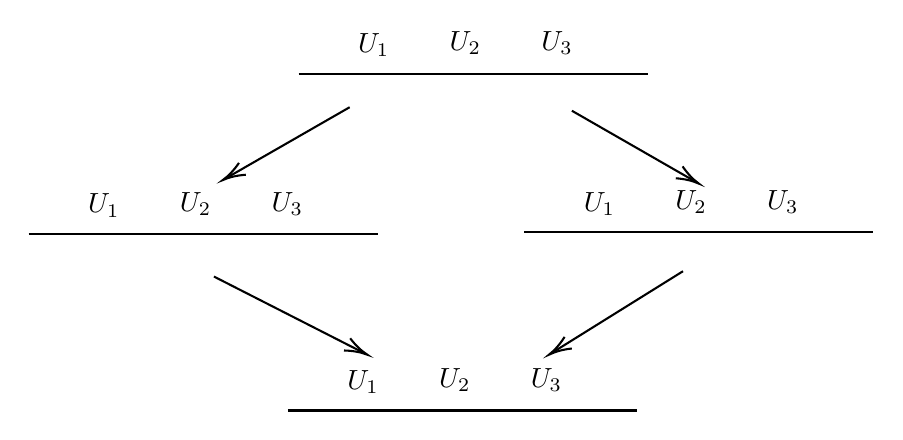
\begin{tikzpicture}[x=0.75pt,y=0.75pt,yscale=-1,xscale=1]
%uncomment if require: \path (0,300); %set diagram left start at 0, and has height of 300

%Straight Lines [id:da5543604292457156] 
\draw    (141,36.09) -- (309.24,36.09) ;
%Straight Lines [id:da4901487194099099] 
\draw    (11,113.41) -- (179.24,113.41) ;
%Straight Lines [id:da1721642744801426] 
\draw    (249.76,112.56) -- (418,112.56) ;
%Straight Lines [id:da22802491317770257] 
\draw    (135.9,198.38) -- (304.14,198.38) ;
%Straight Lines [id:da5450171031412938] 
\draw    (165.64,52.24) -- (106.2,86.36) ;
\draw [shift={(104.47,87.36)}, rotate = 330.14] [color={rgb, 255:red, 0; green, 0; blue, 0 }  ][line width=0.75]    (10.93,-3.29) .. controls (6.95,-1.4) and (3.31,-0.3) .. (0,0) .. controls (3.31,0.3) and (6.95,1.4) .. (10.93,3.29)   ;
%Straight Lines [id:da32782364610967507] 
\draw    (272.7,53.94) -- (332.15,88.06) ;
\draw [shift={(333.88,89.06)}, rotate = 209.86] [color={rgb, 255:red, 0; green, 0; blue, 0 }  ][line width=0.75]    (10.93,-3.29) .. controls (6.95,-1.4) and (3.31,-0.3) .. (0,0) .. controls (3.31,0.3) and (6.95,1.4) .. (10.93,3.29)   ;
%Straight Lines [id:da776515361469394] 
\draw    (100.22,133.81) -- (172.36,170.57) ;
\draw [shift={(174.14,171.48)}, rotate = 207] [color={rgb, 255:red, 0; green, 0; blue, 0 }  ][line width=0.75]    (10.93,-3.29) .. controls (6.95,-1.4) and (3.31,-0.3) .. (0,0) .. controls (3.31,0.3) and (6.95,1.4) .. (10.93,3.29)   ;
%Straight Lines [id:da4544384801263339] 
\draw    (326.23,131.26) -- (263.36,170.42) ;
\draw [shift={(261.66,171.48)}, rotate = 328.09] [color={rgb, 255:red, 0; green, 0; blue, 0 }  ][line width=0.75]    (10.93,-3.29) .. controls (6.95,-1.4) and (3.31,-0.3) .. (0,0) .. controls (3.31,0.3) and (6.95,1.4) .. (10.93,3.29)   ;

% Text Node
\draw (155.46,26.32) node [anchor=north west][inner sep=0.75pt]   [align=left] {$\lb \ \ \ \ \ \ \ \rb$};
% Text Node
\draw (200.5,26.32) node [anchor=north west][inner sep=0.75pt]   [align=left] {$\lb \ \ \ \ \ \ \ \rb$};
% Text Node
\draw (244.68,26.32) node [anchor=north west][inner sep=0.75pt]   [align=left] {$\lb \ \ \ \ \ \ \ \rb$};
% Text Node
\draw (168.16,15.27) node [anchor=north west][inner sep=0.75pt]   [align=left] {$U_1$};
% Text Node
\draw (212.35,14.42) node [anchor=north west][inner sep=0.75pt]   [align=left] {$U_2$};
% Text Node
\draw (256.53,14.42) node [anchor=north west][inner sep=0.75pt]   [align=left] {$U_3$};
% Text Node
\draw (25.46,103.64) node [anchor=north west][inner sep=0.75pt]   [align=left] {$\lb \ \ \ \ \ \ \ \rb$};
% Text Node
\draw (70.49,103.64) node [anchor=north west][inner sep=0.75pt]   [align=left] {$\lb \ \ \ \ \ \ \ \rb$};
% Text Node
\draw (114.68,103.64) node [anchor=north west][inner sep=0.75pt]   [align=left] {$\lb \ \ \ \ \ \ \ \rb$};
% Text Node
\draw (38.16,92.59) node [anchor=north west][inner sep=0.75pt]   [align=left] {$U_1$};
% Text Node
\draw (82.34,91.74) node [anchor=north west][inner sep=0.75pt]   [align=left] {$U_2$};
% Text Node
\draw (126.53,91.74) node [anchor=north west][inner sep=0.75pt]   [align=left] {$U_3$};
% Text Node
\draw (264.22,102.79) node [anchor=north west][inner sep=0.75pt]   [align=left] {$\lb \ \ \ \ \ \ \ \rb$};
% Text Node
\draw (309.26,102.79) node [anchor=north west][inner sep=0.75pt]   [align=left] {$\lb \ \ \ \ \ \ \ \rb$};
% Text Node
\draw (353.44,102.79) node [anchor=north west][inner sep=0.75pt]   [align=left] {$\lb \ \ \ \ \ \ \ \rb$};
% Text Node
\draw (276.92,91.74) node [anchor=north west][inner sep=0.75pt]   [align=left] {$U_1$};
% Text Node
\draw (321.11,90.89) node [anchor=north west][inner sep=0.75pt]   [align=left] {$U_2$};
% Text Node
\draw (365.29,90.89) node [anchor=north west][inner sep=0.75pt]   [align=left] {$U_3$};
% Text Node
\draw (150.37,188.61) node [anchor=north west][inner sep=0.75pt]   [align=left] {$\lb \ \ \ \ \ \ \ \rb$};
% Text Node
\draw (195.4,188.61) node [anchor=north west][inner sep=0.75pt]   [align=left] {$\lb \ \ \ \ \ \ \ \rb$};
% Text Node
\draw (239.58,188.61) node [anchor=north west][inner sep=0.75pt]   [align=left] {$\lb \ \ \ \ \ \ \ \rb$};
% Text Node
\draw (163.06,177.56) node [anchor=north west][inner sep=0.75pt]   [align=left] {$U_1$};
% Text Node
\draw (207.25,176.71) node [anchor=north west][inner sep=0.75pt]   [align=left] {$U_2$};
% Text Node
\draw (251.43,176.71) node [anchor=north west][inner sep=0.75pt]   [align=left] {$U_3$};
% Text Node
\draw (21.2,96.64) node [anchor=north west][inner sep=0.75pt]   [align=left] {{\huge $\lb \ \ \ \ \ \ \ \ \ \ \rb$}};
% Text Node
\draw (304.9,96.64) node [anchor=north west][inner sep=0.75pt]   [align=left] {{\huge $\lb \ \ \ \ \ \ \ \ \ \ \rb$}};
% Text Node
\draw (143.88,183.61) node [anchor=north west][inner sep=0.75pt]   [align=left] {{\huge $\lb \ \ \ \ \ \ \ \ \ \ \ \ \ \ \ \ \ \rb$}};
\end{tikzpicture} \\
&\RA (a\cdot b)\cdot c= a\cdot (b\cdot c).
\eea

\begin{eg}[Chiral QFT] Let $\on{dim }X=2$ (i.e. $X$ is a plane). 
\bea
\tikzset{every picture/.style={line width=0.75pt}} %set default line width to 0.75pt    
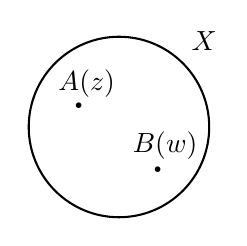
\begin{tikzpicture}[x=0.75pt,y=0.75pt,yscale=-1,xscale=1]
%uncomment if require: \path (0,300); %set diagram left start at 0, and has height of 300

%Shape: Ellipse [id:dp8384382557053032] 
\draw   (66.98,120.35) .. controls (66.98,96.34) and (86.45,76.87) .. (110.46,76.87) .. controls (134.48,76.87) and (153.94,96.34) .. (153.94,120.35) .. controls (153.94,144.37) and (134.48,163.83) .. (110.46,163.83) .. controls (86.45,163.83) and (66.98,144.37) .. (66.98,120.35) -- cycle ;

% Text Node
\draw (79.83,91.45) node [anchor=north west][inner sep=0.75pt]   [align=left] {$A(z)$};
% Text Node
\draw (115.66,121.35) node [anchor=north west][inner sep=0.75pt]   [align=left] {$B(w)$};
% Text Node
\draw (85.82,107.186) node [anchor=north west][inner sep=0.75pt]   [align=left] {{\Huge .}};
% Text Node
\draw (123.79,137.86) node [anchor=north west][inner sep=0.75pt]   [align=left] {{\Huge .}};
% Text Node
\draw (144,73) node [anchor=north west][inner sep=0.75pt]   [align=left] {$X$};
\end{tikzpicture}
\eea

\noindent In holomorphic coordinates, when an operator approach (wind around) the other on $X$, the winding number can be kept track in terms of their Laurent modes:
\bea 
A(z)B(w)=\sum_{m\in \bZ}\frac{\lb A_{(m)}B\rb (w)}{(z-w)^{m+1}}.
\eea
We find $\infty$-ly many ``product'' (binary operation) $\lcb A_{(m)}B \rcb$. Observable algebras then give rise to \textbf{vertex algebras}.
\end{eg}

Observable algebras are developed in the works of:
\begin{itemize}
    \item Beilinson-Drinfeld
    \begin{itemize}
        \item developed factorization algebra to formulate two-dimensional chiral conformal field theory (CFT)
        \item introduced the notion of \emph{chiral homology} (generalize \emph{Hodge homology} in one dimension)
    \end{itemize}
    \item Costello-Gwilliam
    \begin{itemize}
        \item constructed factorization algebras from perturbative renormalization theory, in the \textbf{Batalin-Vilkovisky (BV) formalism} (generalize \emph{BRST formalism} in gauge theory).
    \end{itemize}
\end{itemize}

%\begin{rmk} The geometrical study of QFT are related to index theory: 1-dim. (Atiyah-Singer index theory), 2-dim. (chiral index theory on loop space). (see later) \end{rmk}

\subsection*{BV formalism and homological integration}
    \bea \int \ =\ \text{homology}\eea
\paragraph{Calculus revisited.}
    Let $M$ be a compact oriented manifold of $\on{dim} M=n$. Many constructions of integration on manifolds can be understood from de Rham complex
    $\lb \Omega^\blt(M), d\rb$. Consider the integration map 
    \bea
    \int_M: \Omega^\blt(M) \to \bR,\qquad
    \alpha\in \Omega^n(M) \mapsto \int_M \alpha. \eea
    Observe that the $n$-th de Rham cohomology group
    $H^n_{dR}(M) =\bR$. This implies that 
    \bea
    \int_M \ = \ H^n_{dR}. \eea
    The integration map is now
    \bea
    \Omega^n(M) \to H^n_{dR}(M),\qquad
    \alpha \mapsto [\alpha].
    \eea
    This means that we can learn calculus by the algebraic structure on de Rham complex, even we do not know anything about measure theory. However, there is a problem of understanding $H^n_{dR}(M)$ when $n\to\infty$ as in QFT.
    
\paragraph{BV approach.}
    Define \textbf{polyvector fields}
    \bea 
    \on{PV}^\blt(M) =\bigoplus_k \on{PV}^k(M)\coloneqq \bigoplus_k \Gamma \lb M,\ \asym^k TM\rb.
     \eea
    Let $\Omega$ be a fixed volume form on $M$. We can naturally identify
    \bea
    \on{PV}^k(M) \lra \Omega ^{n-k}(M),\qquad
    \mu\in \on{PV}^k(M) \lra \mu \lrcorner \Omega.
    \eea
    Locally, if $\Omega=e^\varphi dx^1\wedge \cdots \wedge dx^n$, $\mu=\mu^{i_1\cdots i_k} \partial_{i_1}\wedge \cdots \wedge \partial_{i_k}$, then
    \bea \mu \lrcorner\Omega= \sum \pm \mu^{i_1\cdots i_k} e^\varphi dx^1 \wedge \cdots \wedge \widehat{dx^{i_1}}\wedge \cdots \wedge\widehat{dx^{i_k}} \wedge \cdots \wedge dx^n. \eea
    
    %%%%%%%%%%%%%%%%%%%%%%%%%%%%%%%%%%%%
    The identification above leads to 
    \bea
    \begin{tikzcd}
    \Omega^{0} \ar[r, "d"] \ar[dd, "\simeq"] 
    & \Omega^{1} \ar[r, "d"] \ar[dd, "\simeq"] 
    & \cdots \ar[r,"d"] & \Omega^{n} \ar[dr, "\int"] \ar[dd, "\simeq"] & \\
     & & & & \bR \\
    PV^{n} \ar[r, "\Delta"]
    & PV^{n-1} \ar[r, "\Delta"]
    & \cdots \ar[r, "\Delta"] & PV^{0} \ar[ur, "\int_{\on{BV}}"] & 
    \end{tikzcd}
    \eea
where
$\Delta: \on{PV}^k \to \on{PV}^{k-1}$ is a divergence operator with respect to $\Omega$. $\Delta$ is called the \textbf{BV operator}.
For example, 
$\Delta: \on{PV}^1=\on{Vect}(M) \to \on{PV}^0=C^\infty(M)$ is the usual divergence.

$\int_{\on{BV}}$ is the \textbf{BV integration}, which is a map:
\bea \int_{\on{BV}}: \on{PV}^0 \to \bR,\qquad 
f \mapsto \int f\Omega.
\eea
Homologically $\int_{\on{BV}}$ can be identified with $H^0_{\on{BV}}$.
Here ``$\on{dim} (M)$'' does not appear. The problem of integration is transferred to construct $\Delta$, which has a convenient formulation at least in perturbative QFT.
In $\infty$-dimensions (as in QFT), renormalization helps to construct $\Delta$ which leads to \textbf{homological integration}.

\paragraph{Explicit form of $\Delta$.}
Locally in $U$, let $\lcb x_i\rcb_{i=1}^n$ be local coordinates and $\Omega=e^{f(x)}dx^1\wedge \cdots \wedge dx^n$ be the volume form. Introduce the vector fields $\partial_i=\frac{\partial}{\partial x_i}$, then the polyvector field is \bea \on{PV}(U)=C^\infty(U) [\partial_1, \cdots, \partial_n],\eea
where $\partial_i$'s are anticommuting: $\partial_i \partial_j =- \partial_j \partial_i$. 
Let us write $\theta_i=\partial_i$ (\textit{note}: this is a vector field, NOT an differential operator), then a local section $\mu\in \on{PV}(X)$ can be written as a function of $x^i$, $\theta_i$:
\bea
\mu=\mu (x^i, \theta_i)
\eea
with $x^ix^j=x^j x^i$ and $\theta_i \theta_j =- \theta_j \theta_i$.
Let $\frac{\partial}{\partial x^i}$ be the derivative with respect to $x^i$  and $\frac{\partial}{\partial \theta_i}$ be the derivative with respect to $\theta_i$ (from the left). Then the BV operator is given locally by 
\bea
\Delta = \sum_i \frac{\partial}{\partial x^i} \frac{\partial}{\partial \theta_i}
+\sum_i (\partial_i f) \frac{\partial}{\partial \theta_i}
\eea
which looks like a second order operator (it is easy to check that $\Delta^2=0$). This is in contrast with de Rham differential $d$, which is a first order differential
operator. Note that the first term looks like a Laplacian, but it is NOT. $\theta_i$ is an odd variable. Hence, $\Delta$ is sometimes called an \emph{odd Laplacian}.

\begin{eg}[$\frac{\partial}{\partial \theta_i}$ operator]
\bea\frac{\partial}{\partial \theta_1}(\theta_1\theta_2) &=\theta_2,\\
\frac{\partial}{\partial \theta_1}(\theta_2\theta_1) &=- \frac{\partial}{\partial \theta_1}(\theta_1\theta_2)=-\theta_2.
\eea
\end{eg}

\begin{eg}[Singularity theory]
Consider the $n$-th dimensional complex space $\bC^n$. Let $f: \bC^n\to \bC$ be a polynomial in $n$ variables with an isolated critical pint at 0:
\bea \on{Crit}(f)=\lcb 0\rcb.\eea
We consider holomorphic/polynomial polyvector fields
\bea \cA =\bC[z^i, \theta_i], \quad
\theta_i \theta_j =- \theta_j \theta_i.\eea
Let the BV operator be
\bea \Delta=\hbar \sum_{i=1}^n \frac{\partial}{\partial z^i} \frac{\partial}{\partial \theta_i}
+\sum_i (\partial_i f) \frac{\partial}{\partial \theta_i}. \eea
\begin{itemize}
    \item The space of quantum observables $\on{Obs}^q=H^\blt (\cA \llb  \hbar\rrb,\Delta)$ is isomorphic to a formal completion of the Brieskorn lattice.
    \item 
    The quantum observable (or Brieskorn lattice) plays an important role of Hodge filtration (which is related to $\hbar$-filtration) in singularity theory.
    \item The BV-integration models the oscillatory integral 
    \bea\lan \cO\ran=\int_{\mathcal{L}} d^n z\ \cO e^{f/\hbar},\eea where $\mathcal{L}$ is a Lefschetz thimble.
\end{itemize}
\end{eg}

\noindent \textsc{Reference}: \cite{Li:2017exk}.
